\documentclass[11pt,letterpaper]{article}
\usepackage[lmargin=1in,rmargin=1in,tmargin=1in,bmargin=1in]{geometry}
\usepackage{../style/homework}
\usepackage{../style/commands}
\setbool{quotetype}{false} % True: Side; False: Under
\setbool{hideans}{true} % Student: True; Instructor: False

% Logical Circuits
\usepackage{circuitikz}
\usetikzlibrary{shapes.gates.logic.US,shapes.gates.logic.IEC}

% -------------------
% Content
% -------------------
\begin{document}
\homework{2: Due 01/04}{If the presence of electricity can be made visible in any part of the circuit, I see no reason why intelligence may not be transmitted instantaneously by electricity.}{Samuel Morse}

% Problem 1
\problem{10} Construct the on/off table for the following circuit: 
	\[
	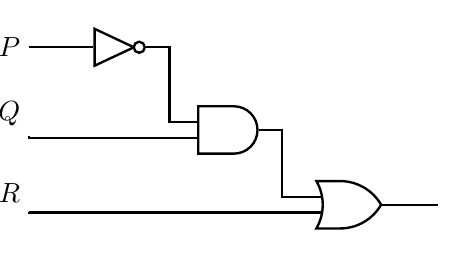
\begin{tikzpicture}
	\node (p) at (0,2.85) {\hspace{-0.5cm}$P$};
	\node (q) at (0,2) {\hspace{-0.5cm}$Q$};
	\node (r) at (0,1) {\hspace{-0.5cm}$R$};
	
	\node[not gate US, draw, line width= 0.03cm] at (1,2.85) (not1) {};
	\node[and gate US, draw, line width= 0.03cm] at (2.5,1.80) (and1) {};
	\node[or gate US, draw, line width= 0.03cm] at (4,0.85) (or1) {};
	 
	\draw[line width= 0.03cm] (p) |- (not1.input);
	\draw[line width= 0.03cm] (not1.output) -- ([xshift=0.3cm]not1.output) |- (and1.input 1);
	\draw[line width= 0.03cm] (and1.output) --  ([xshift=0.3cm]and1.output) |- (or1.input 1);
	\draw[line width= 0.03cm] (q) |- (and1.input 2);
	\draw[line width= 0.03cm] (r) |- (or1.input 2);
	\draw[line width= 0.03cm] (or1.output) -- ([xshift=0.7cm]or1.output);
	\end{tikzpicture}
	\]



\newpage



% Problem 2
\problem{10} Find the logical expression corresponding to the following circuit:
	\[
	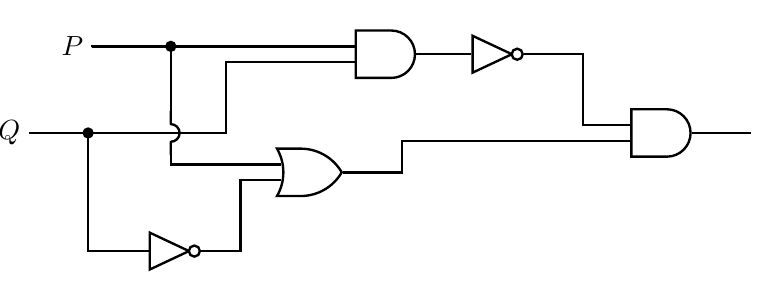
\begin{tikzpicture}
	\node (p) at (0.3,3.1) {\hspace{-0.5cm}$P$};
	\node (q) at (-0.5,2) {\hspace{-0.5cm}$Q$};
	
	\node[and gate US, draw, line width= 0.03cm] at (4,3) (and1) {};
	\node[not gate US, draw, line width= 0.03cm] at (1.2,0.5) (not1) {};
	\node[or gate US, draw, line width= 0.03cm] at (3,1.5) (or1) {};
	\node[not gate US, draw, line width= 0.03cm] at (5.3,3) (not2) {};
	\node[and gate US, draw, line width= 0.03cm] at (7.5,2) (and2) {};
	
	\draw[line width= 0.03cm] (q) to[short,-*] (0.25,2) |- (not1.input);
	\draw[line width= 0.03cm] (not1.output) -- ([xshift=0.5cm]not1.output) |- (or1.input 2);
	\draw[line width= 0.03cm] (q) |- (2,2) |- (and1.input 2);
	\draw[line width= 0.03cm] (and1.output) |- (not2.input);
	\draw[line width= 0.03cm] (not2.output) --  ([xshift=0.75cm]not2.output) |- (and2.input 1);
	\draw[line width= 0.03cm] (and2.output) -- ([xshift=0.75cm]and2.output);
	\draw[line width= 0.03cm] (p) |- (and1.input 1);
	\draw[line width= 0.03cm] (p) to[short,-*] (1.3,3.1);
	
	\node[scale=2,rotate=-90] at (1.3,2) [line width=0.03cm,jump crossing] (cross) {};
	\draw[line width= 0.03cm] (1.3,3.1) |- (cross.west);
	\draw[line width= 0.03cm] (cross.east) |- (or1.input 1);
	
	\draw[line width= 0.03cm] (or1.output) |- ([xshift=0.75cm]or1.output) |- (and2.input 2);
	\end{tikzpicture}
	\]



\newpage



% Problem 3
\problem{10} Find the circuit corresponding to the following logical expression:
	\[
	(P \wedge Q) \vee (\neg P \wedge R)
	\]



\newpage



% Problem 4
\problem{10} Find a logical expression corresponding to the following input/output table: \par
	\begin{table}[h]
	\centering
	\begin{tabular}{c|c|c|c}
	$P$ & $Q$ & $R$ & ? \\ \hline
	$1$ & $1$ & $1$ & $0$ \\
	$1$ & $1$ & $0$ & $0$ \\
	$1$ & $0$ & $1$ & $0$ \\
	$1$ & $0$ & $0$ & $1$ \\
	$0$ & $1$ & $1$ & $0$ \\
	$0$ & $1$ & $0$ & $1$ \\
	$0$ & $0$ & $1$ & $1$ \\
	$0$ & $0$ & $0$ & $0$ 
	\end{tabular}
	\end{table}



\newpage



% Problem 5
\problem{10} Watch Sebastian League's \href{https://www.youtube.com/watch?v=QZwneRb-zqA&ab_channel=SebastianLague}{``Exploring How Computers Work''} and \href{https://www.youtube.com/watch?v=I0-izyq6q5s&ab_channel=SebastianLague}{``How Do Computers Remember?''} on YouTube. Being as detailed as possible, explain what you learned and how it relates to the course material.  


\end{document}